\documentclass[pdflatex,sn-mathphys-num]{sn-jnl}% Math and Physical Sciences Numbered Reference Style

\usepackage{graphicx}%
\usepackage{multirow}%
\usepackage{amsmath,amssymb,amsfonts}%
\usepackage{amsthm}%
\usepackage[title]{appendix}%
\usepackage{xcolor}%
\usepackage{textcomp}%
\usepackage{manyfoot}%
\usepackage{booktabs}%
\usepackage{algorithm}%
\usepackage{algorithmicx}%
\usepackage{algpseudocode}%
\usepackage{listings}%

\providecommand{\code}[1]{\texttt{#1}}%
\algrenewcommand\algorithmicrequire{\textbf{Input:}}
\algrenewcommand\algorithmicensure{\textbf{Output:}}

\theoremstyle{thmstyleone}%
\newtheorem{theorem}{Theorem}%
\newtheorem{proposition}[theorem]{Proposition}%

\theoremstyle{thmstyletwo}%
\newtheorem{example}{Example}%
\newtheorem{remark}{Remark}%

\theoremstyle{thmstylethree}%
\newtheorem{definition}{Definition}%

\raggedbottom

\begin{document}
\graphicspath{{figures/}}

\title[Adaptive Identification and Tracking]{Adaptive Candidate Routing for Distributed Occupant Recognition Across Multiple Building IoT-enabled Smart Spaces}

\author[1]{\fnm{Yadhu Vipin } \sur{Madhilakath Madathil}}\email{yadhuvipin12@gmail.com }
\equalcont{These authors contributed equally to this work.}

\author[1]{\fnm{D Aditya } \sur{Kiran}}\email{akdattingal@gmail.com}
\equalcont{These authors contributed equally to this work.}

\author[1]{\fnm{Arjun} \sur{Rajesh}}\email{arjunrajesh59@gmail.com}

\author*[1]{\fnm{Lakshmi } \sur{Mohan}}\email{lakshmimohan@am.amrita.edu }

\affil*[1]{\orgdiv{Department of Computer Science and Engineering }, \orgname{Amrita School of Computing, Amrita Vishwa
Vidyapeetham}, \orgaddress{\street{Amritapuri}, \city{Kollam}, \postcode{690525}, \state{Kerala}, \country{India}}}

%\affil[2]{\orgdiv{Department}, \orgname{Organization}, \orgaddress{\street{Street}, \city{City}, \postcode{10587}, \state{State}, \country{Country}}}

%\affil[3]{\orgdiv{Department}, \orgname{Organization}, \orgaddress{\street{Street}, \city{City}, \postcode{610101}, \state{State}, \country{Country}}}


\abstract{This work proposes a multi-building biometric-embedding routing mechanism for occupant identification and tracking across indoor environments in IoT-enabled smart spaces. Centralized galleries raise privacy concerns, while distributed galleries incur overhead in locating the appropriate building before recognition. The proposed approach models the environment using a Distributed State Transition System (DSTS), where states represent occupant presence probabilities, events represent biometric recognition, and transitions describe state evolution. Each building shares a Bloom filter constructed from locality-sensitive hashing (LSH) codes of its registered occupants. After a face is captured the system creates L codes. Those codes are checked against every filter and the system gives a rank to each building. Only the top‑ranked buildings then check the face against their stored reference embeddings. In tests that used 500 identities from CASIA-WebFace spread across 10 buildings. Repeated 20 times with random assignments the system correctly identified 92.81 percent of routed visitors. In contrast a centralized recognition system reached 95.50 percent. A flexible strategy that asks buildings when the rank list is unclear reaches 92.95 percent for routed visitors but it asks an average of only 2.54 buildings for each query. The rate of positives from the filter is 3.54 percent, higher than the set limit of 1 percent and this happens because of collisions in the LSH codes. The size of the communication payload is only estimated, not measured. The system has not yet been tested for encryption or, for visitors that are unknown.}
\keywords{Occupant identification and tracking, Distributed state transition system, Smart spaces, Locality-sensitive hashing, Bloom filter, Face recognition}


\maketitle


\section{Introduction}

Camera networks are in wide use across IoT-enabled smart spaces for monitoring occupants and supporting occupant-specific, building-level services~\cite{SM2022, hou2017}. These services require dependable occupant identification and tracking so that facial observations are linked to the right individuals. When services span several buildings, identity resolution depends on how biometric reference data are stored and accessed across them. A centralized architecture keeps one common database of reference face embeddings, whereas a distributed architecture keeps the biometric reference data within each building. Centralization places sensitive biometric data in a single location and introduces a potential single point of failure, while distribution removes the dependence on a central repository but makes it harder to identify occupants across building boundaries~\cite{mohan2020}.

In a distributed setting, an individual registered with one building can be regarded as a visitor when entering another building in which the individual is not registered. Identifying such visitors is challenging because the potential visitor set of a building may include occupants registered across other buildings and may approach the size of the overall registered population. Identifying visitors may require either sharing reference embeddings between buildings or searching the local databases of several buildings, at the cost of higher computational overhead and the potential exposure of additional biometric data.

To address this challenge, this work proposes a decentralized face recognition strategy that uses locality-sensitive hashing (LSH) and Bloom filters to route query embeddings to candidate buildings while retaining reference embeddings locally. Each building-level state transition system (BSTS) shares a Bloom filter constructed from the LSH codes of its registered occupants' face embeddings with all other buildings. The query embedding ranks the candidate BSTSs, and identity is verified by local angular-distance voting only in the selected buildings. The framework is evaluated on 500 CASIA-WebFace identities distributed over ten simulated buildings, and the results are averaged over 20 random assignments. For routed visitors, the adaptive policy attains 92.95\% correct identification while contacting an average of 2.54 buildings per query, compared with 95.50\% for centralized search.

The rest of the paper is structured as follows. Section~\ref{sec:related} surveys related work on occupant identification, distributed state transition systems, biometric privacy, and distributed query routing. Section~\ref{sec:methodology} presents the proposed framework, covering LSH encoding, Bloom-filter construction, candidate routing, and local verification. Section~\ref{sec:setup} describes the experimental setup and evaluation metrics, Section~\ref{sec:results} reports the results, and Section~\ref{sec:discussion} discusses them. Section~\ref{sec:conclusion} concludes, states the limitations of the current evaluation, and outlines future work.


%=====================================================================

\section{Related Work}
\label{sec:related}

Occupant identification and tracking in IoT-enabled smart spaces is based on camera or radio-frequency (RF) sensing~\cite{mohan2020,WZSYGWLLHSC2025}, and indoor localization over Wi-Fi can use weighted trilateration on dual-band signals~\cite{MSSAB2019}. Cameras support unobtrusive facial identification, including tracking across non-overlapping cameras~\cite{nair2021}, and optimizing camera placement improves the coverage of surveillance networks~\cite{SM2022}. In multi-building deployments, identity verification that relies on a central store of biometric data raises computational and privacy concerns~\cite{mohan2020}.

State transition models represent occupant tracking through states, recognition events, and transition functions~\cite{MJG2011}. The DSTS extends this approach to multiple buildings, each represented by a BSTS, where registered occupants are recognized against the local database of their building and visitors are resolved through a centralized master list~\cite{mohan2020}. Related work also addresses video synopsis~\cite{NGA2022} and quantitative metrics for smart spaces~\cite{MMJ2025}. Privacy-preserving biometric methods include Bloom-filter protection of iris templates~\cite{rathgeb2014}, and Marzani et al.~\cite{marzani2026} in their work combine face features, fuzzy extractors, and homomorphically encrypted Bloom filters to count individuals across locations. In contrast, our proposed work uses LSH codes and per-BSTS Bloom filters to route a captured embedding towards candidate buildings on the basis of approximate similarity, while the reference embeddings remain local.

The proposed routing combines established techniques. Random-hyperplane LSH produces binary codes that preserve angular similarity~\cite{charikar2002}, multi-probe lookup inspects neighboring codes to improve recall without additional hash tables~\cite{lv2007}, and Bloom filters~\cite{bloom1970} offer compact approximate set membership, with bit positions obtained by double hashing~\cite{kirsch2006}. Related work on distributed search includes Summary Cache~\cite{fan2000}, which uses Bloom filters to find the web proxies likely to hold a requested object; the partitioning-based routing of nearest-neighbor search requests to the relevant data shards studied by Gottesb{\"u}ren et al.~\cite{gottesbueren2024}; and Semord~\cite{wang2026semord}, which organizes similar vectors in a decentralized overlay through learned hashing and exchanged summaries. Unlike approaches that rely on vector placement or shared vector summaries, the proposed framework shares only compact Bloom filters of LSH codes and does not distribute reference face embeddings. To the best of our knowledge, this combination has not previously been evaluated for occupant identification across multiple BSTSs.


% ============================================================
% METHODOLOGY
% ============================================================


\section{Methodology}
\label{sec:methodology}

\subsection{System Model and Assumptions}
\label{subsec:system_model}

This work extends the visitor identification step of the DSTS framework described in~\cite{mohan2020}. The state transition function is defined as $\Delta:\mathcal{S} \times \mathcal{E} \rightarrow \mathcal{S}$, describing how an environment changes state following a biometric recognition event. An occupant is recognized by comparing the captured face embedding with the local database of the building where they are registered. Visitors, who are registered occupants of other buildings, are identified using a visitor list containing building-specific visitor embeddings to generate the corresponding event. A visitor is an individual observed in a building where they are not registered and whose reference embeddings are maintained elsewhere. The objective is to reduce the comparisons required for visitor identification by locating the building holding the visitor's reference embeddings without searching every building's database.

The environment consists of $B$ buildings, each with a BSTS maintaining a local reference database $\mathcal{D}_b$, where $b\in\{1,\ldots,B\}$, containing the face embeddings of its registered occupants. Each BSTS constructs a Bloom filter from its occupants' LSH codes and shares it with all other BSTSs, so that every building holds the filters of all $B$ buildings while keeping $\mathcal{D}_b$ local. If a face captured in a building is not accepted by any occupant of that building, the capturing building checks the captured embedding against the filters of the other buildings, ranks them, and selects a shortlist. It sends the captured embedding to the shortlisted buildings, each of which verifies it against its local reference embeddings and returns the outcome; if none accepts, the system abstains. A centralized system that stores all reference embeddings in a single database serves as the performance baseline. Communication between buildings is assumed to be protected by the deployment infrastructure. Because LSH codes and Bloom filters are compact routing representations rather than encryption mechanisms, no formal privacy guarantee is claimed.

\subsection{LSH Encoding}
\label{subsec:lsh_encoding}

Faces are detected and aligned with SCRFD-10GF~\cite{guo2022} and embedded with a pretrained ArcFace model~\cite{deng2019} (InsightFace \code{buffalo\_l}), for reference and captured images alike. A raw embedding $\hat{\mathbf{e}}^{\mathrm{raw}}\in\mathbb{R}^{512}$ is normalized, centered with the reference-derived mean $\bar{\mathbf{x}}$, and normalized again:
\begin{equation}
    \hat{\mathbf{e}}
    =
    \frac{
        \frac{\hat{\mathbf{e}}^{\mathrm{raw}}}{\|\hat{\mathbf{e}}^{\mathrm{raw}}\|_2}
        - \bar{\mathbf{x}}
    }{
        \left\|
        \frac{\hat{\mathbf{e}}^{\mathrm{raw}}}{\|\hat{\mathbf{e}}^{\mathrm{raw}}\|_2}
        - \bar{\mathbf{x}}
        \right\|_2
    }.
    \label{eq:embedding_preprocessing}
\end{equation}
The $R$ preprocessed reference embeddings $\hat{\mathbf{e}}_{u,1},\ldots,\hat{\mathbf{e}}_{u,R}$ of a registered occupant $u$ give a normalized centroid
\begin{equation}
    \mathbf{z}_u
    =
    \frac{
        \sum_{r=1}^{R}\hat{\mathbf{e}}_{u,r}
    }{
        \left\|\sum_{r=1}^{R}\hat{\mathbf{e}}_{u,r}\right\|_2
    },
    \label{eq:identity_centroid}
\end{equation}
and LSH codes are computed from $\mathbf{z}_u$ for registered occupants and from $\hat{\mathbf{e}}$ for captured faces.

The codes use random hyperplanes~\cite{charikar2002}: vectors $\mathbf{w}_{\ell,k}\in\mathbb{R}^{512}$ ($\ell<L$, $k<K$), drawn once from a standard Gaussian distribution and shared by all buildings, define $L$ slots of $K$ bits. The bit $h_{\ell,k}$ records the side of the hyperplane on which the embedding lies, and the $K$ bits of slot $\ell$ form an integer code:
\begin{equation}
    h_{\ell,k}(\hat{\mathbf{e}}) =
    \begin{cases}
        1, & \mathbf{w}_{\ell,k}^\top\hat{\mathbf{e}} \geq 0,\\
        0, & \text{otherwise},
    \end{cases}
    \qquad
    c_\ell(\hat{\mathbf{e}}) = \sum_{k=0}^{K-1} 2^{k}\, h_{\ell,k}(\hat{\mathbf{e}}) \in \{0,\ldots,2^K-1\}.
    \label{eq:lsh_bit}
\end{equation}
Each code is tagged with its slot identifier,
\begin{equation}
    s_\ell(\hat{\mathbf{e}})
    =
    \ell 2^K + c_\ell(\hat{\mathbf{e}}),
    \label{eq:tagged_code}
\end{equation}
so that codes from different slots are never confused; an embedding is represented by $L$ tagged codes (Algorithm~\ref{alg:build}). Embeddings at angle $\theta$ agree on one bit with probability $1-\theta/\pi$~\cite{charikar2002}, on all $K$ bits of a slot with probability $(1-\theta/\pi)^K$, and on at least one of the $L$ slots with probability
\begin{equation}
    P_{\mathrm{match}}(\theta)=1-\Bigl(1-\bigl(1-\tfrac{\theta}{\pi}\bigr)^{K}\Bigr)^{L}.
    \label{eq:slot_agreement}
\end{equation}
$P_{\mathrm{match}}(\theta)$ is high for the small angles of the same person and low for the large angles between different people; a larger $K$ reduces chance agreement and a larger $L$ raises the agreement of the same identity.

\subsection{Bloom-Filter Construction and Sharing}
\label{subsec:bloom_filter}

Each building $b$ inserts the $L$ tagged items of each of its $N$ registered occupants into its Bloom filter $F_b$~\cite{bloom1970}, so $n=N\cdot L$ items are inserted (Algorithm~\ref{alg:build}). A Bloom filter reports an item as absent or as possibly present, so a positive can be false. For a target false-positive probability $f^*$, the filter size $m$ (in bits) and the number of hash positions $\kappa$ are
\begin{equation}
    m =
    \left\lceil
    -\frac{n\ln f^*}{(\ln 2)^2}
    \right\rceil,
    \qquad
    \kappa =
    \operatorname{round}
    \left(\frac{m}{n}\ln 2\right).
    \label{eq:bloom_size}
\end{equation}
The $\kappa$ positions of an item $s$ come from double hashing~\cite{kirsch2006} of two 64-bit hash values and a shared salt, and $\textsc{Insert}(F_b,s)$ sets them in $F_b$. Each building shares its Bloom filter with the others before recognition begins. No reference embeddings are exchanged; only the filters are shared in advance. A positive response only qualifies a building as a candidate.

\begin{algorithm}[!t]
\footnotesize
\caption{LSH encoding and Bloom-filter construction at building $b$}
\label{alg:build}
\begin{algorithmic}[1]
\Require Raw reference embeddings $\hat{\mathbf{e}}^{\mathrm{raw}}_{u,r}$ of $N$ occupants ($R$ each), mean $\bar{\mathbf{x}}$, vectors $\mathbf{w}_{\ell,k}$, $K$, $L$ (Section~\ref{subsec:lsh_encoding}), $f^*$ (Section~\ref{subsec:bloom_filter})
\Ensure Bloom filter $F_b$, shared with all other buildings
\State $n\gets N\cdot L$; compute $m$ and $\kappa$ from $n$ and $f^*$ \Comment{Eq.~\eqref{eq:bloom_size}}
\State $F_b\gets$ bit array of $m$ zeros
\For{each registered occupant $u=1,\dots,N$}
  \State $\hat{\mathbf{e}}_{u,r}\gets$ preprocess $\hat{\mathbf{e}}^{\mathrm{raw}}_{u,r}$ for $r=1,\dots,R$ \Comment{Eq.~\eqref{eq:embedding_preprocessing}}
  \State $\mathbf{z}_u\gets$ normalized sum of $\hat{\mathbf{e}}_{u,1},\dots,\hat{\mathbf{e}}_{u,R}$ \Comment{Eq.~\eqref{eq:identity_centroid}}
  \For{each slot $\ell=0,\dots,L-1$}
    \State $h_{\ell,k}\gets[\mathbf{w}_{\ell,k}^\top\mathbf{z}_u\geq 0]$ for $k=0,\dots,K-1$; $c_\ell\gets\sum_{k}2^{k}h_{\ell,k}$ \Comment{Eq.~\eqref{eq:lsh_bit}}
    \State $s_\ell\gets\ell 2^K+c_\ell$; \textsc{Insert}$(F_b,s_\ell)$ \Comment{Eq.~\eqref{eq:tagged_code}; set the $\kappa$ bit positions}
  \EndFor
\EndFor
\State share $F_b$ with all other buildings; \Return $F_b$
\end{algorithmic}
\end{algorithm}

\subsection{Routing and Verification}
\label{subsec:routing_verification}

For a captured embedding, the building where the face is captured computes the $L$ tagged codes of Eq.~\eqref{eq:tagged_code} and checks them against the Bloom filter of every other building. Multi-probe lookup~\cite{lv2007} extends this check beyond the codes themselves. Let $\mu_{\ell,k}=|\mathbf{w}_{\ell,k}^\top\hat{\mathbf{e}}|$ be the margin of bit $k$ in slot $\ell$. Bits with a small margin lie close to the hyperplane and are the most likely to differ between two embeddings of the same person, so the $P$ bit positions $k_1,\ldots,k_P$ with the smallest margins are flipped one at a time, giving the probe codes $c_\ell^{(i)}=c_\ell\oplus 2^{k_i}$ for $i=1,\ldots,P$ in addition to $c_\ell$ itself; $P$ is the number of extra probes per slot. Only the captured embedding is probed; the codes inserted for registered occupants are unchanged. The routing score $A_b$ of a building is the number of slots for which at least one of the $P+1$ probed items is reported present (each slot counts at most once), and the $S$ highest-ranked buildings form the shortlist, where $S$ is the shortlist size, with ties resolved by building index. The score gap $g$ is the difference between the two highest scores.

At a shortlisted building, the captured embedding is compared with the local reference embeddings by angular distance. A reference contributes a vote when its angle to the captured embedding is at most the threshold $\tau$, so the vote count of a registered occupant $u$ is $v_u=|\{r:\angle(\hat{\mathbf{e}},\hat{\mathbf{e}}_{u,r})\leq\tau\}|$. The occupant with the most votes (ties broken by the smallest angle $\theta_u$) is the local candidate and is accepted only if its vote count reaches the minimum number of votes $V$. This procedure, $\textsc{Verify}(b,\hat{\mathbf{e}})$, returns the local candidate, its vote count and its smallest angle. Routing determines which reference databases are consulted, and the local reference embeddings provide the evidence for accepting or rejecting an identification.

Three verification policies determine which shortlisted buildings are contacted. Under the default policy, all shortlisted buildings verify the captured embedding, and the accepting building with the most votes is selected (ties are broken by the smaller angle, then by routing rank). Under sequential verification, the shortlisted buildings are contacted in routing order and verification stops at the first building that accepts; this contacts fewer buildings but may accept an incorrect identity from a building ranked above the correct one. Under adaptive verification, the score gap $g$ is compared with a threshold $g_0$: if $g\le g_0$ the ranking is ambiguous and all shortlisted buildings verify the captured embedding, and otherwise the sequential rule is used. In all policies the system abstains if no contacted building reaches $V$ votes. The values of $P$, $S$, $V$ and $g_0$ are given in Section~\ref{sec:setup} and are not claimed to be optimal.

% ============================================================
% EXPERIMENTAL SETUP
% ============================================================

\section{Experimental Setup}
\label{sec:setup}

\subsection{Dataset and Protocol}

The experiments use 500 identities of CASIA-WebFace~\cite{yi2014}, a public face dataset collected from the web. The identities are divided at random into $B=10$ buildings of 50 occupants each, and each building enrolls its occupants by storing their reference embeddings in its local database and building its Bloom filter from them. Each identity contributes 20 enrolled reference images and 20 held-out test images, which are disjoint and fixed across runs, giving 10,000 reference and 10,000 test embeddings. Each run simulates one day of 10,000 recognition events, one per test image: 8,000 local events, in which an occupant is captured in the building where the occupant is registered, and 2,000 visitor events, in which an occupant is captured in a building where the occupant is not registered. A visitor is first compared with the 50 occupants of the capturing building. If no occupant of that building reaches the vote threshold, the captured embedding is checked against the Bloom filters of the other nine buildings and routed as described in Section~\ref{subsec:routing_verification}. The evaluation is closed-set, as every captured face belongs to an enrolled occupant; unknown individuals are not evaluated.


\subsection{Parameters and Compared Methods}

The mean embedding $\bar{\mathbf{x}}$ and angle threshold $\tau$ are estimated from reference images only. The threshold $\tau=80.43^{\circ}$ minimizes the combined false-reject rate for genuine pairs (7.7\%) and false-accept rate for impostor pairs (0.5\%). It applies to individual image pairs and is not a calibrated error rate for the voting rule.

For each $K$, the smallest $L$ giving same-identity reference-image pairs a 0.90 probability of agreeing in at least one slot is selected, averaged over measured pair angles. This heuristic is conservative because routing compares captured embeddings with occupant centroids. The leave-one-out mean angle is $46.2^{\circ}$ for centroids and $60.1^{\circ}$ between images. Applying the same rule to centroids gives $L=43$ for $K=11$. The selected setting, $K=11$ and $L=122$, gives genuine code agreement of 0.0187 per slot and impostor agreement of 0.062 across all slots. This setting was chosen after examining test-image accuracy.

The remaining parameters are $P=3$, $S=5$, $V=12$ votes out of 20 references, $g_0=5$, and $f^*=0.01$, giving $n=6100$ items per filter. Values of $P$ from 0 to 7 are also tested. The centralized baseline searches the 450 enrolled identities not registered in the capturing building, using the same $\tau$, vote threshold, and tie-breaking rule as the distributed methods, without building-level routing.

Results are averaged over 20 random seeds. Each seed changes the building assignments, LSH hyperplanes, Bloom-filter salt, and simulated visitor events; the embeddings, reference/test split, and $\tau$ remain fixed. The 95\% confidence half-widths use Student's $t$-distribution with 19 degrees of freedom and describe variation across runs, not across people, datasets, or deployments.


\subsection{Evaluation Metrics}

The outcomes are computed for routed visitors, that is, visitors that no occupant of the capturing building accepts; visitors accepted by the capturing building are counted separately. Each routed visitor receives exactly one outcome. If a building accepts, the attempt is correct when the accepted occupant is the true one and misidentified otherwise. If no building reaches $V$ votes, the attempt is a verification rejection when the true building was shortlisted and a routing abstention otherwise. The policies are compared by the mean number of buildings contacted per attempt and the share of attempts contacting all five shortlisted buildings. Bloom-filter quality is measured by the effective false-positive rate, obtained by testing the enrolled items of the other nine buildings against the filter of each building. Communication is computed analytically from the measured contacts (Section~\ref{sec:cost}); latency and traffic were not measured.

% ============================================================
% RESULTS
% ============================================================

\section{Results}
\label{sec:results}

\subsection{Distributed versus Centralized Identification}

Of the 2,000 visitor events per run, $65\pm4$ (3.3\%) are accepted by an occupant of the capturing building, and the remaining 1,935 are routed; the percentages below refer to routed visitors. Local events are recognized correctly in 95.96\% of cases. Centralized search over the 450 identities achieves 95.50\% correct identification, with 1.31\% misidentification and 3.19\% abstention. Under the default distributed policy, which verifies all five shortlisted buildings, correct identification is 92.81\%, misidentification is 1.44\%, and the remaining attempts are divided between 1.97\% verification rejections and 3.78\% routing abstentions. Correct identification is 2.69 percentage points lower than for the centralized baseline, and in 3.78\% of attempts the building holding the correct reference is not among the five shortlisted buildings. Multi-probe routing reduces these routing abstentions: they fall from 6.86\% without additional probes ($P=0$) to 3.78\% at $P=3$, and correct identification rises from 89.31\% to 92.81\%. Larger values of $P$ yield smaller improvements (93.33\% at $P=7$) while the lookups per filter, $L(1+P)$, grow linearly, so $P=3$ is adopted as a trade-off.

\subsection{Verification Policies}

Table~\ref{tab:adaptive} compares centralized search with the three policies on the routed visitors, and Fig.~\ref{fig:results} shows the buildings that the policies contact. The policies contact 1.49 (sequential), 2.54 (adaptive) and 5.00 (verify all five) of the nine candidate buildings on average, reductions of 83\%, 72\% and 44\% relative to contacting all nine. Sequential verification is the cheapest but raises misidentification to 2.06\%, because an incorrect building ranked above the correct one sometimes accepts first. Verifying all five buildings lowers misidentification to 1.44\%. The adaptive policy achieves 92.95\% correct identification and 1.30\% misidentification, and all five shortlisted buildings are contacted for 37.6\% of attempts. The paired per-seed difference between adaptive verification and verifying all five buildings is $0.14\pm0.04$ points (95\% half-width, adaptive better in 19 of 20 seeds), a small improvement in these simulations, and centralized search remains $2.55\pm0.16$ points above adaptive verification. All three policies abstain on the same attempts.

\begin{figure}[!t]
\centering
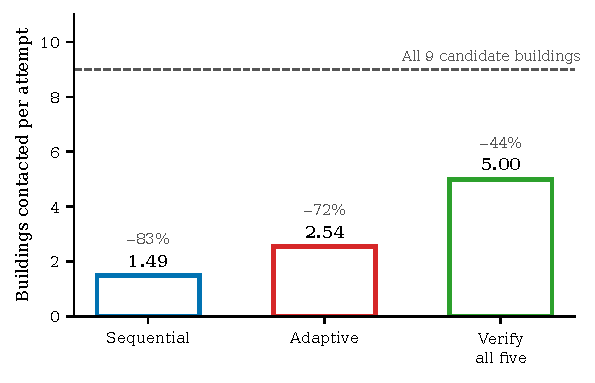
\includegraphics[width=0.55\textwidth]{figures/fig2_results.pdf}
\caption{Buildings contacted per identification attempt for routed visitors at 10 buildings (mean over 20 seeds). The dashed line marks the nine candidate buildings, which is the number contacted without routing; the percentages give the reduction relative to it.}
\label{fig:results}
\end{figure}

\begin{table}[!t]
\caption{Results for routed visitor events at 10 buildings and a shortlist of five (visitors accepted by the capturing building are excluded): mean over 20 seeds with 95\% confidence half-widths ($\pm$). The centralized baseline is a single central endpoint, so no building count is given. Payload is the estimated captured-embedding traffic per attempt.}\label{tab:adaptive}%
\begin{tabular}{@{}lcccc@{}}
\toprule
Method & Correct (\%) & Misidentified (\%) & Buildings & Payload (KB) \\
\midrule
Centralized (450 identities) & $95.50 \pm 0.25$ & $1.31 \pm 0.10$ & -- & 2.0 \\
Sequential & $92.19 \pm 0.28$ & $2.06 \pm 0.12$ & 1 & 3.1 \\
Adaptive & $92.95 \pm 0.28$ & $1.30 \pm 0.11$ & 3 & 5.2 \\
Verify all five & $92.81 \pm 0.29$ & $1.44 \pm 0.10$ & 5 & 10.2 \\
\bottomrule
\end{tabular}
\end{table}

\subsection{Bloom-Filter False-Positive Rate}
\label{sec:fpr}

The Bloom filters are configured for a false-positive probability of 1\%, whereas the effective rate, measured by testing the enrolled items of the other nine buildings against each filter, is $3.54 \pm 0.02\%$. Without a Bloom array, $2.61 \pm 0.02\%$ of the items of other buildings already equal an enrolled item in the same slot, close to the 2.41\% expected if the codes of 50 occupants were evenly distributed over $2^{11}=2048$ values, whereas the Bloom array alone yields $0.94 \pm 0.01\%$ on random integers that were never inserted. The excess over the configured target comes from collisions between the LSH codes of different occupants and not from the Bloom array.

\subsection{Communication Cost}
\label{sec:cost}

The estimates use message sizes and the measured number of buildings contacted, and they exclude protocol headers, replies, filter updates and synchronization. A 512-dimensional float32 embedding occupies 2,048 bytes, so an attempt contacting $q$ buildings generates $2048q$ bytes. Centralized search sends the embedding once to a central endpoint (2.0~KB), which holds all reference embeddings (20.5~MB). The distributed design shares ten Bloom filters of 7.3~KB each (73~KB in total), held by every building, and each building keeps 2.05~MB of reference embeddings locally. An attempt costs 3.1~KB under sequential verification, 5.2~KB under adaptive verification and 10.2~KB when all five shortlisted buildings are contacted, against 18.4~KB for contacting all nine candidate buildings, and routing requires $(B-1)\cdot L(1+P)=4{,}392$ filter lookups, which grow linearly with the number of buildings.

% ============================================================
% DISCUSSION
% ============================================================


\section{Discussion}
\label{sec:discussion}

The difference in accuracy between distributed and centralized search comes from three sources: routing failures (3.78\%), where the correct building is not shortlisted; verification failures (1.97\%), where the correct building rejects the identity; and misidentifications (1.44\%), where another identity is accepted. Routing failures account for the largest share of the gap, so improving the ranking and the shortlist coverage would be more effective than replacing the local verifier. Under sequential verification, the first building that reaches the vote threshold is accepted, so an incorrect building ranked above the correct one increases misidentification; verifying all five buildings avoids this because the candidate with the most votes is selected, at the price of additional contacts. Adaptive verification follows the sequential rule when the gap between the two highest routing scores exceeds $g_0$ and verifies all shortlisted buildings when the scores are close. This reduces misidentification to 1.30\% with 2.54 contacts on average, and its small advantage over verifying all five buildings is consistent across seeds. Bloom-filter false positives introduce additional candidate matches, which local verification may reject, but they can also alter the building ranking and the shortlist, so they may influence identification outcomes as well as communication cost. In addition, 3.3\% of visitors are accepted by the capturing building before routing, so this error cannot be corrected by the proposed mechanism.

The shared filters also raise a privacy concern. Since their LSH codes preserve similarity, someone with access to the filters and public hash parameters could check whether a face produces matches for a particular building and infer that the person may be registered there. Although reference embeddings are not shared, this potential exposure was not evaluated. Access controls, keyed hashing, or encryption could help protect the filters, but these measures remain future work.


% ============================================================
% CONCLUSION
% ============================================================


\section{Conclusion}
\label{sec:conclusion}

This work explored a way to route visitor identification requests across multiple buildings using Bloom filters built from LSH codes, while keeping reference face embeddings within their respective buildings. The experiments evaluated visitor routing and verification, but did not establish complete occupant tracking, correct state transitions, or formal privacy protection. Using 500 CASIA-WebFace identities across 10 buildings, verification of the five shortlisted buildings achieved 92.81\% correct identification for routed visitors, compared with 95.50\% for centralized search. The adaptive policy achieved 92.95\% accuracy while contacting an average of 2.54 of the nine candidate buildings, with an estimated payload of 5.2~KB per attempt. These savings come with reduced recall when the correct building is not shortlisted, while LSH code collisions also increase the effective false-positive rate beyond the Bloom-filter target. Future work will examine larger and more diverse populations, improved candidate ranking, protection of shared filters, recognition of unknown visitors, and measured communication costs.

These results are limited to 500 identities from one public dataset in a closed-set setting with 10 buildings, the parameters $K$ and $P$ were selected after examining test-image accuracy without a separate validation set, and 3.3\% of visitors are accepted by the capturing building before routing and cannot be recovered by the proposed mechanism. Communication costs are estimated from message sizes rather than measured, and encryption, unknown visitors, and a security analysis of the shared filters were not evaluated, so no formal privacy guarantee is established.


\bmhead{Acknowledgement}

The authors gratefully acknowledge Sri Mata Amritanandamayi Devi (Amma), Chancellor, Amrita Vishwa Vidyapeetham, for her inspiration and for providing financial support for the Article Processing Charges (APC) of this publication.

\bibliography{akd}% akd.bib

\end{document}
